\chapter{Appendix 1: Rare Anchored motifs in social support}

%\newcounter{row}
\makeatletter
\@addtoreset{subfigure}{row}
\makeatother
% **************************** Define Graphics Path **************************

\graphicspath{{Chapter3/plots/}{Chapter3/plots/figures/}{Chapter3/plots/Zscore/}}

I evaluate the prevalence of all the Anchored Triadic motifs as defined in Chapter \ref{chap:structure_support}. As explored by previous studies~\cite{shizuka2015network,shizuka2012social,holland1976local,doi:10.1177/104649647100200201}, the social-tie structures and certain triadic motifs are predictors of social hierarchy in communities. Albeit these studies looked at community structures of Apes and tribal populations, they act as a very peculiar proxies for understanding how communities in the wild evolve. The important point to note here is that graphs that emerge from conversations, may not be synonymous to the graphs that form due to actual social ties. But in the context of a conversation, the interactions between peers can be assumed to be a purely transactional tie. 

The internet has opened up new mechanisms of formation of these ties. And at that, the mechanisms seem to generate new patterns of conversations, based on the kind of interaction the participants of a community perform. To that end both the supportive and baseline communities exhibits a dearth of transitive triads like \textsl{030T} and \textsl{210C}, which are more prevalent in real life communities with hierarchies

One of the most interesting outcome of this exercises, which I failed to pursue further is the complete lack of triadic closures. Triadic closure has been a very important aspect of studies around online social capital. The key premise here is that a weak tie can act as a bridge between two disjoint nodes in a community. However, in the context of conversation structures, this phenomenon seems to be completely absent from the picture.


\begin{figure}[htb]
    \renewcommand{\thesubfigure}{\arabic{row}.\alph{subfigure}}%
    \centering
    \setcounter{row}{1}%
    \subfloat[]{
        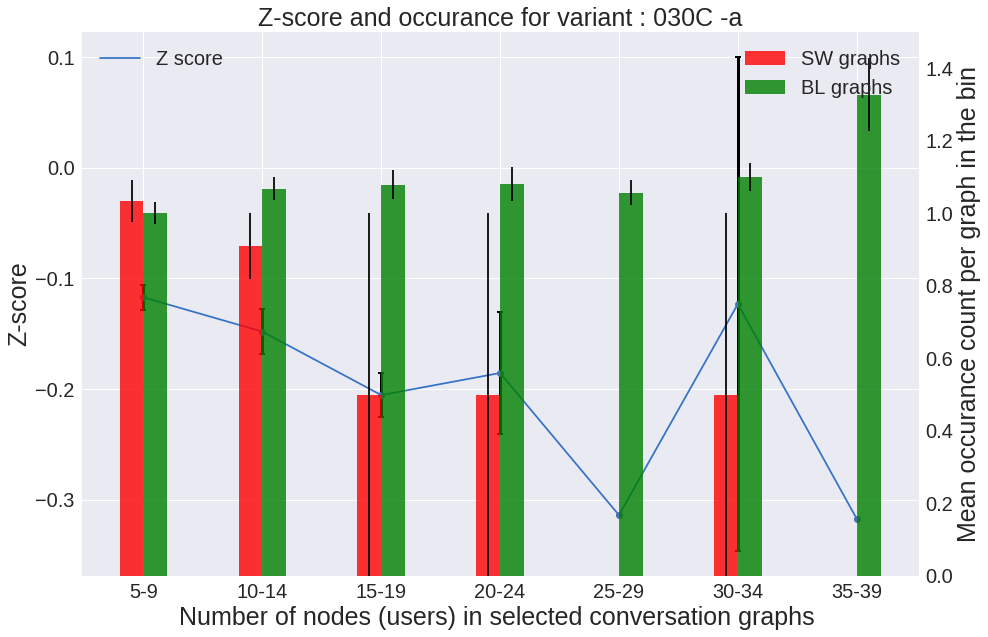
\includegraphics[width=0.33\textwidth]{030C-a.png}
    }
    \subfloat[]{
        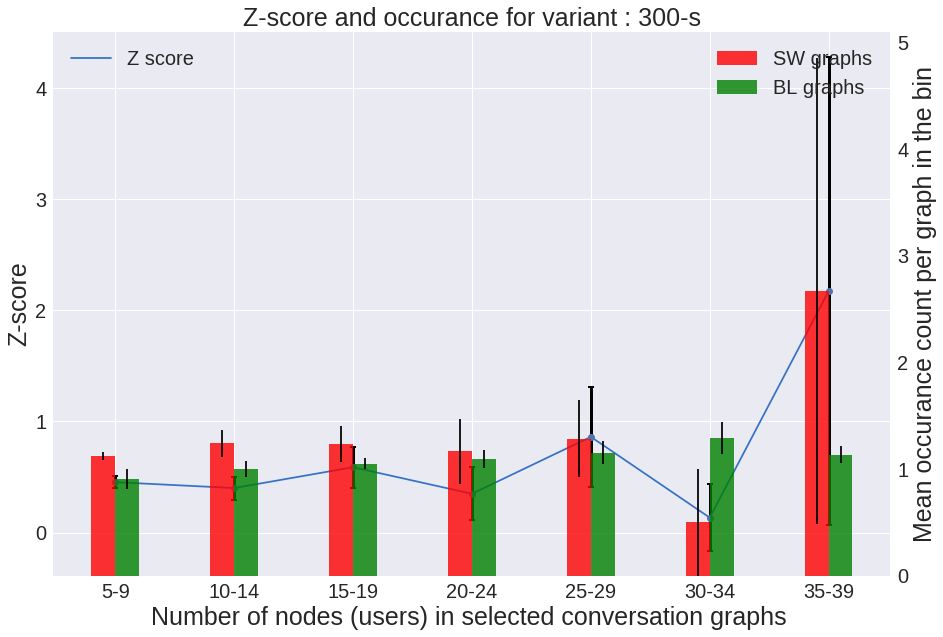
\includegraphics[width=0.33\textwidth ]{300-s.png}
    }
    \subfloat[]{
        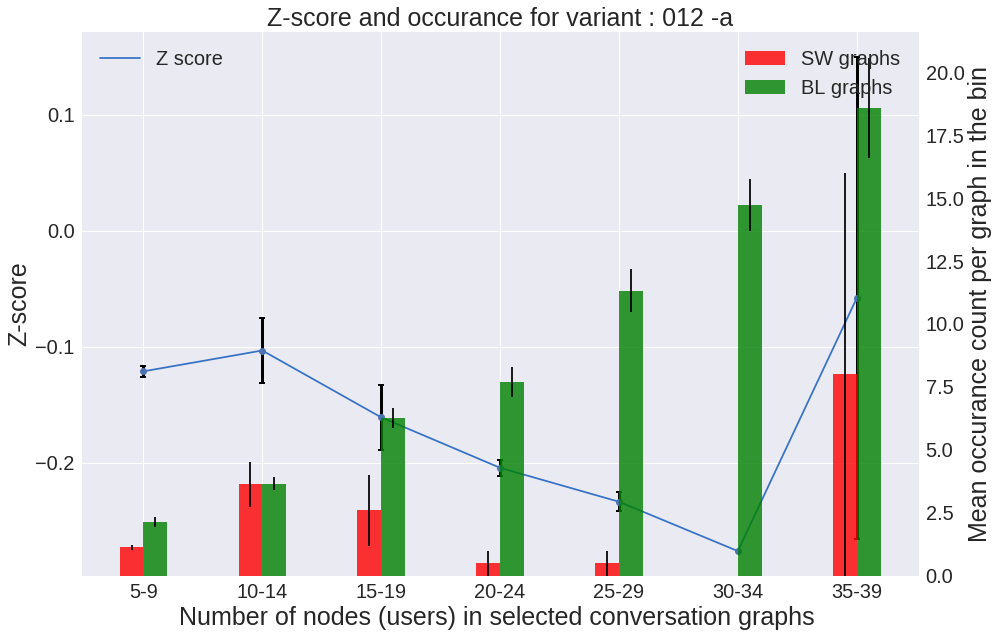
\includegraphics[width=0.33\textwidth]{012-a.png}
    }
    
    
    \stepcounter{row}%
    \subfloat[]{
        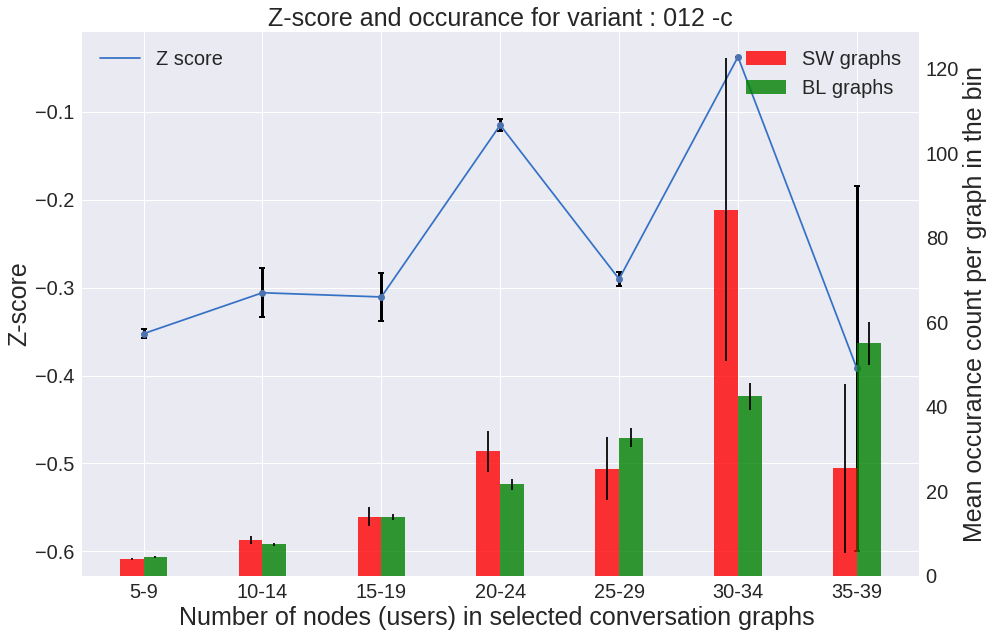
\includegraphics[width=0.33\textwidth ]{012-c.png}
    }
    \subfloat[]{
        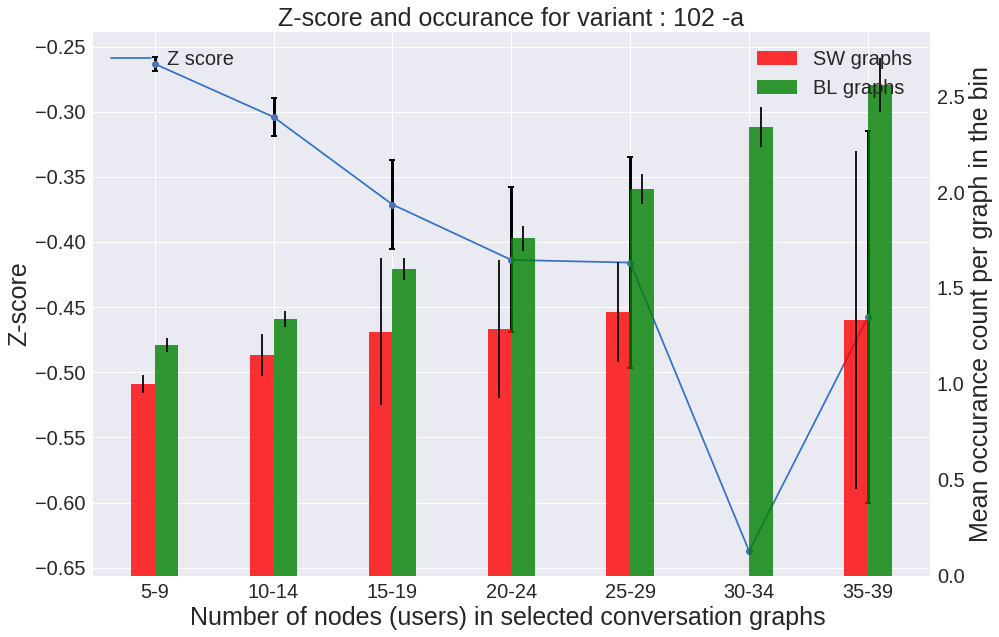
\includegraphics[width=0.33\textwidth]{102-a.png}
    }
    \subfloat[]{
        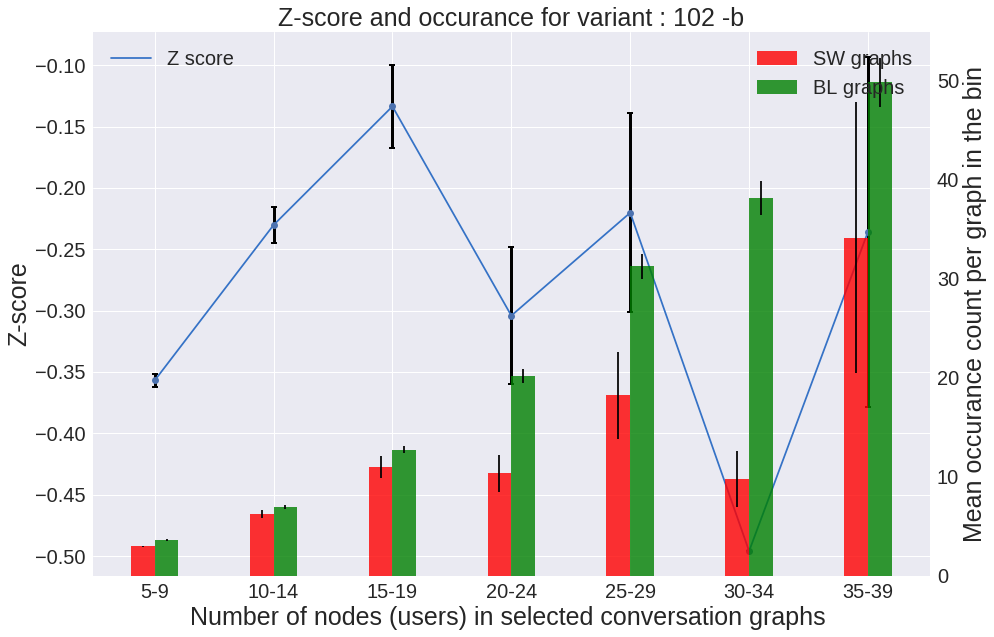
\includegraphics[width=0.33\textwidth]{102-b.png}
    }
    
    \stepcounter{row}%
    \subfloat[]{
        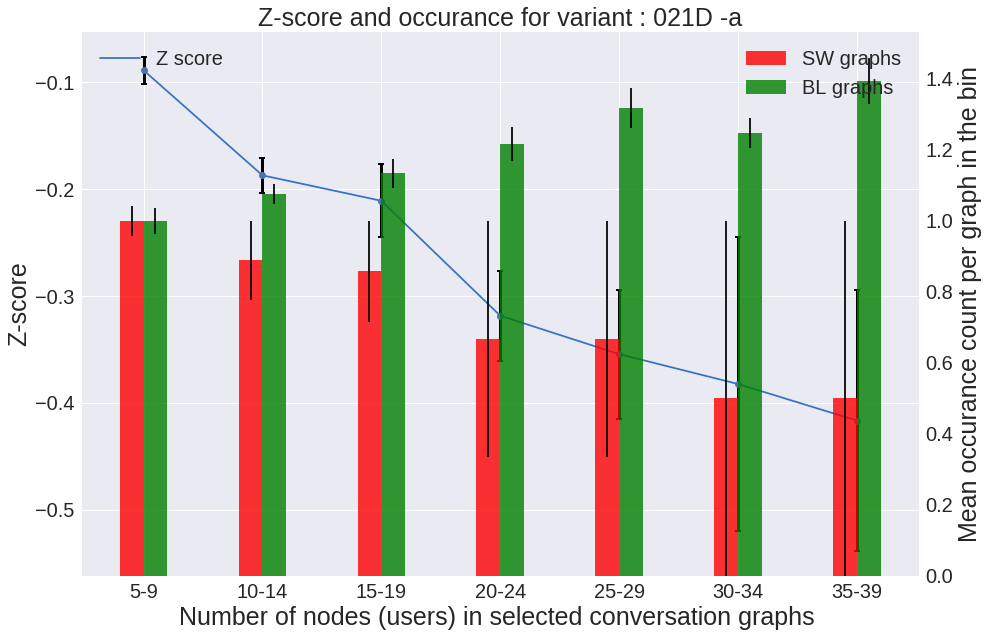
\includegraphics[width=0.33\textwidth ]{021D-a.png}
    }
    \subfloat[]{
        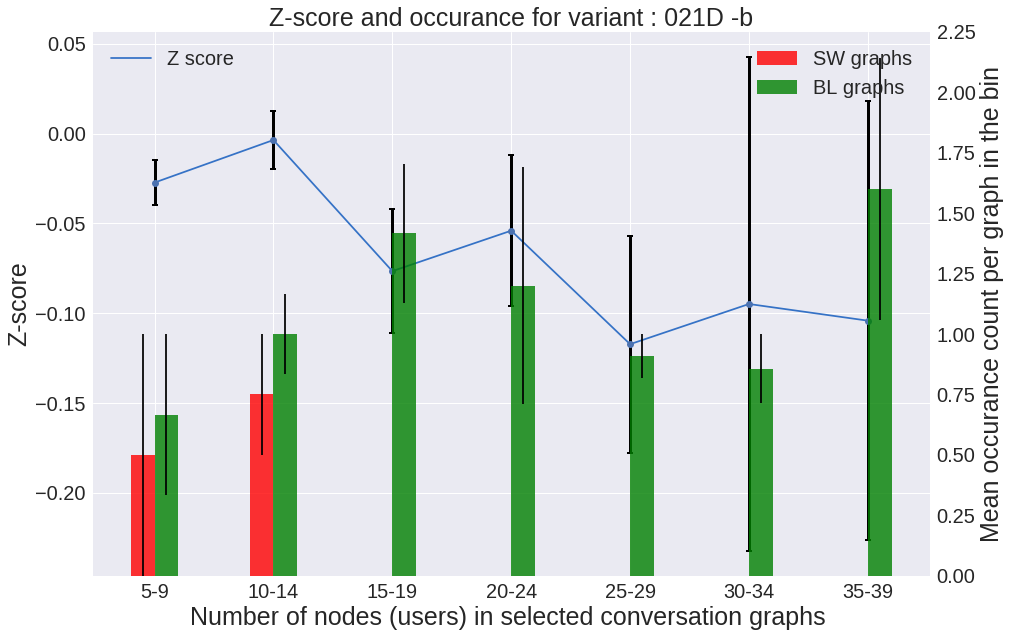
\includegraphics[width=0.33\textwidth ]{021D-b.png}
    }
    \subfloat[]{
        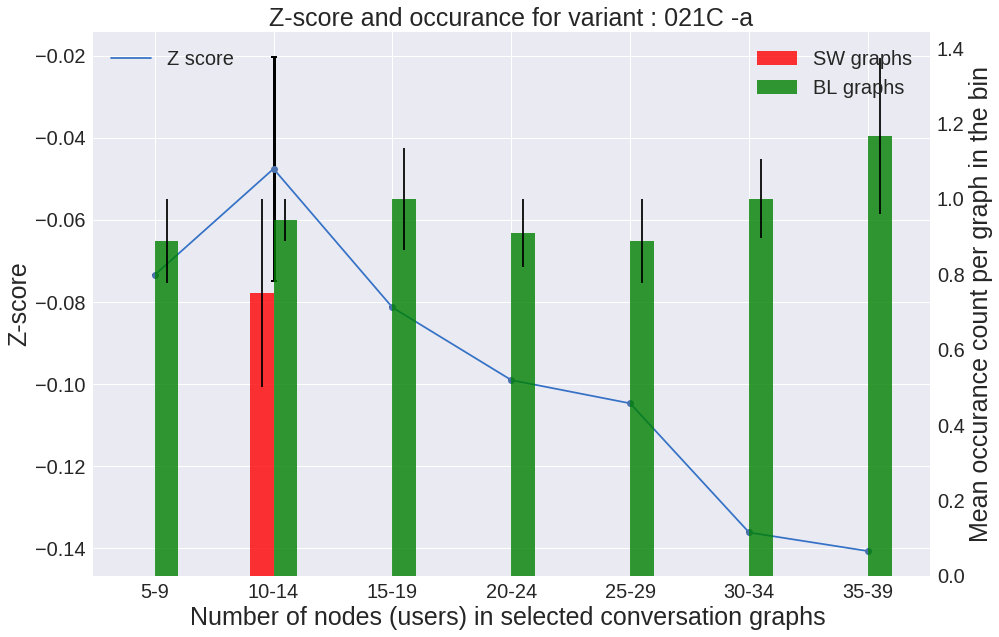
\includegraphics[width=0.33\textwidth]{021C-a.png}
    }
    
    
    \stepcounter{row}%
    \subfloat[]{
        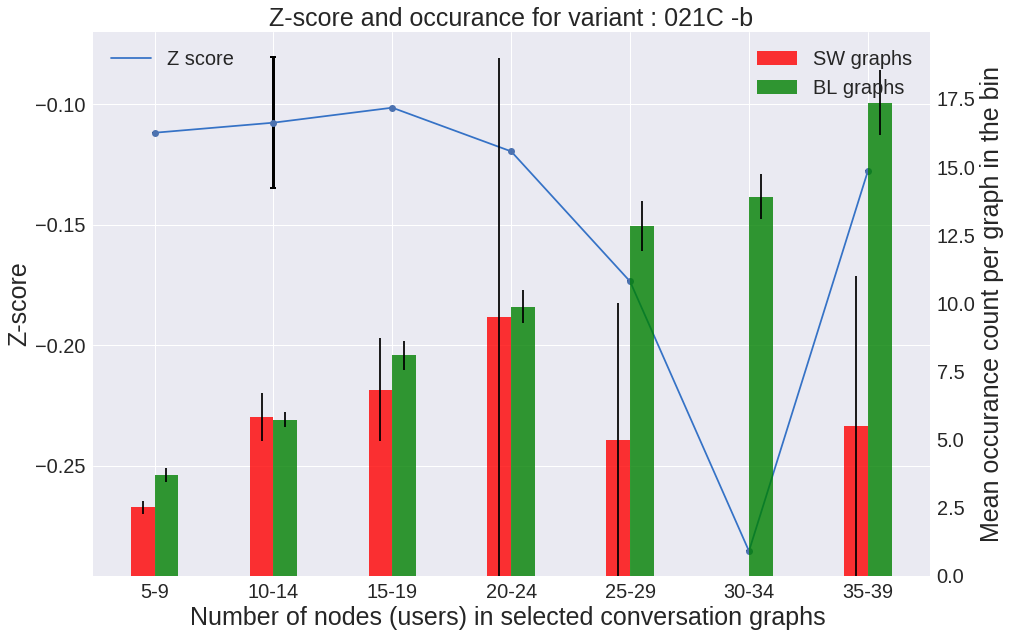
\includegraphics[width=0.33\textwidth]{021C-b.png}
    }
    \subfloat[]{
        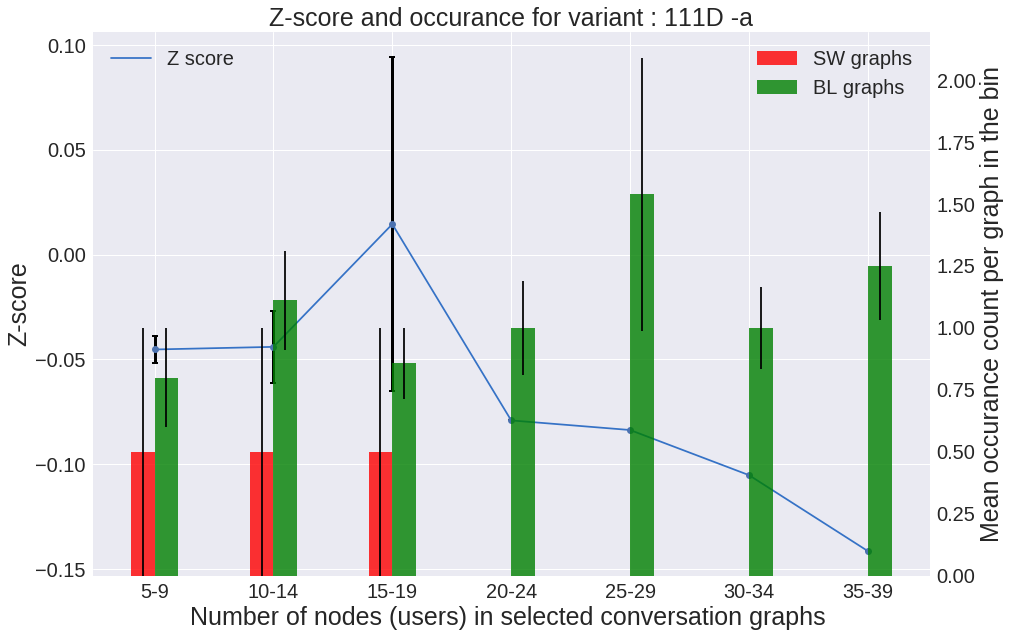
\includegraphics[width=0.33\textwidth ]{111D-a.png}
    }
    \subfloat[]{
        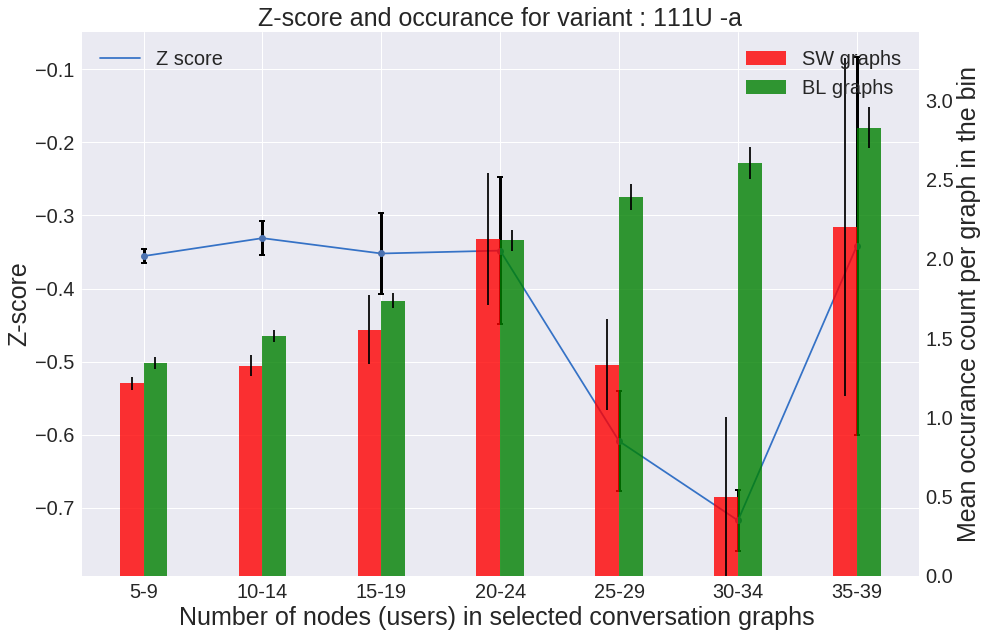
\includegraphics[width=0.33\textwidth ]{111U-a.png}
    }
    
    
    \stepcounter{row}%
    \subfloat[]{
        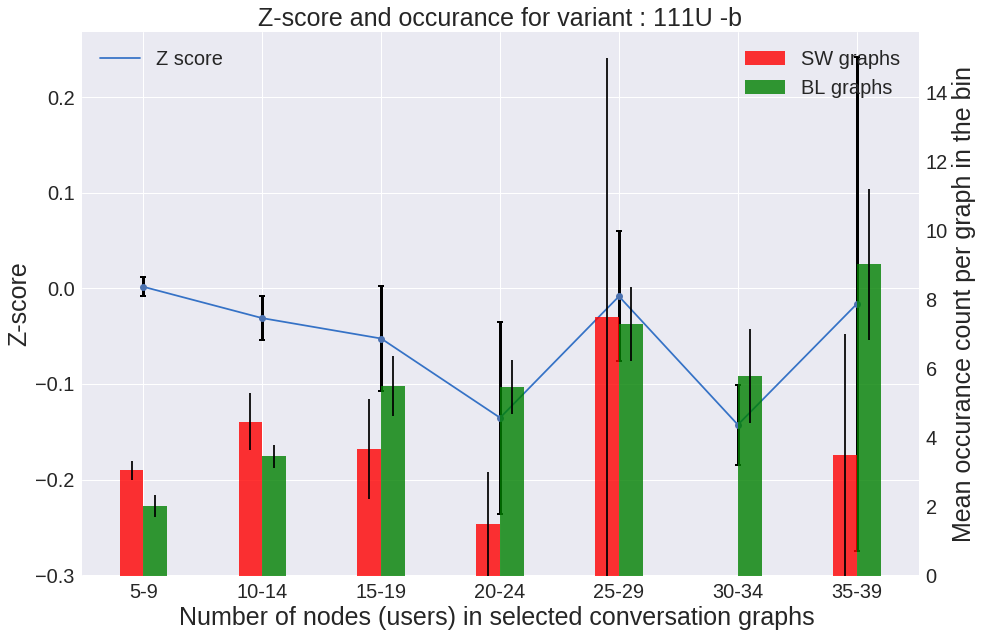
\includegraphics[width=0.33\textwidth]{111U-b.png}
    }
    \subfloat[]{
        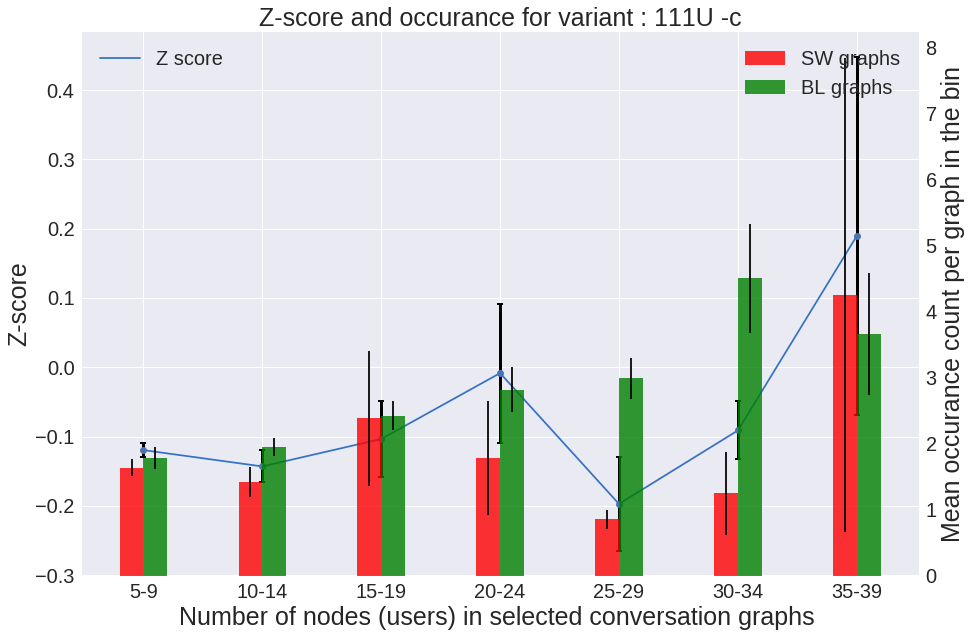
\includegraphics[width=0.33\textwidth ]{111U-c.png}
    }
    \subfloat[]{
        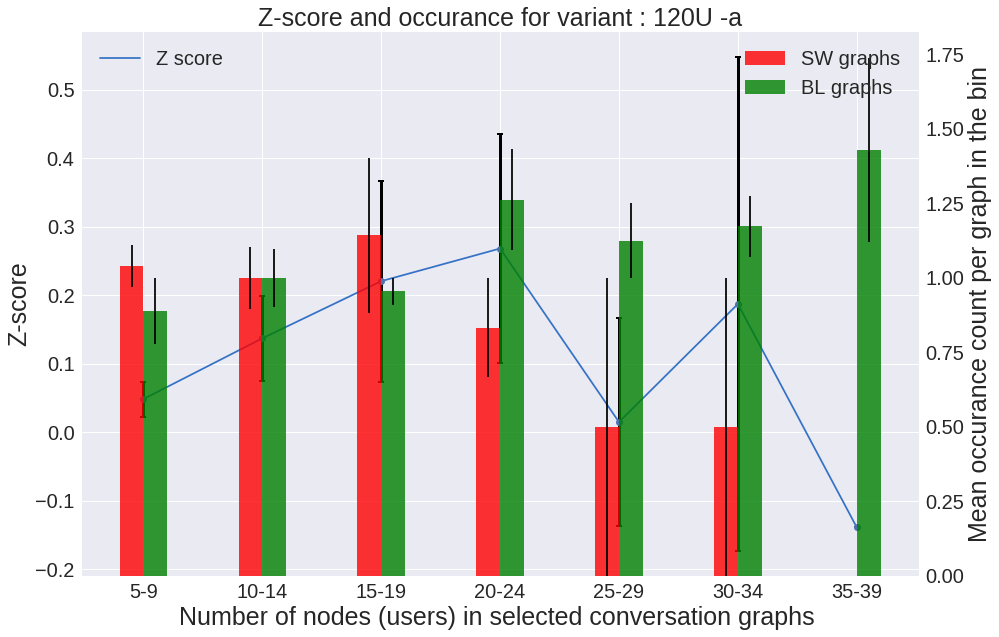
\includegraphics[width=0.33\textwidth]{120U-a.png}
    }
\end{figure}


\begin{figure}[htb]\ContinuedFloat
    \renewcommand{\thesubfigure}{\arabic{row}.\alph{subfigure}}%
    \centering
    
    \setcounter{row}{6}%
    \subfloat[]{
        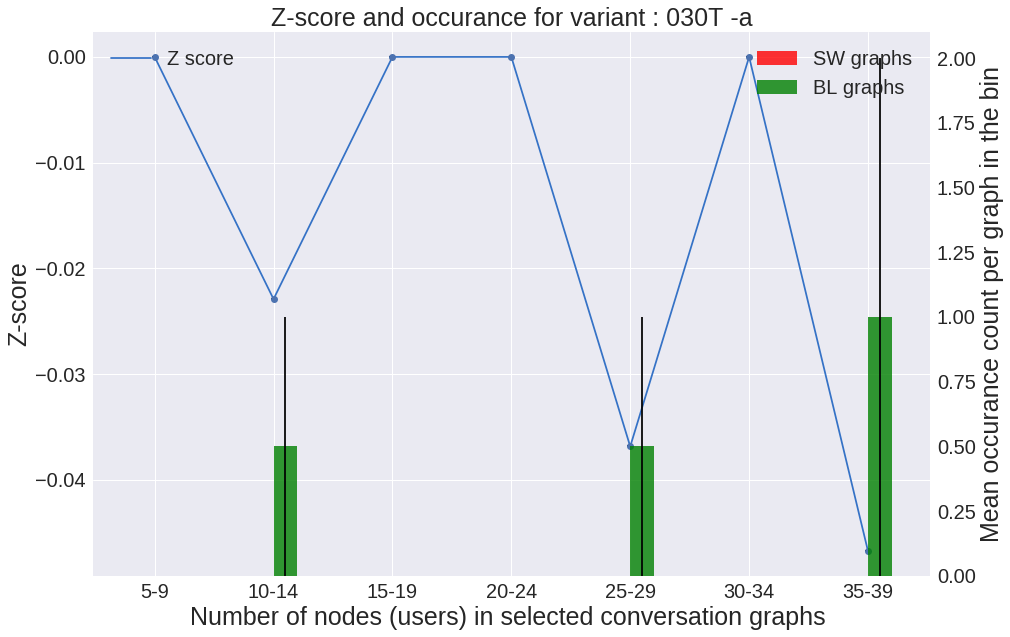
\includegraphics[width=0.33\textwidth]{030T-a.png}
    }
    \subfloat[]{
        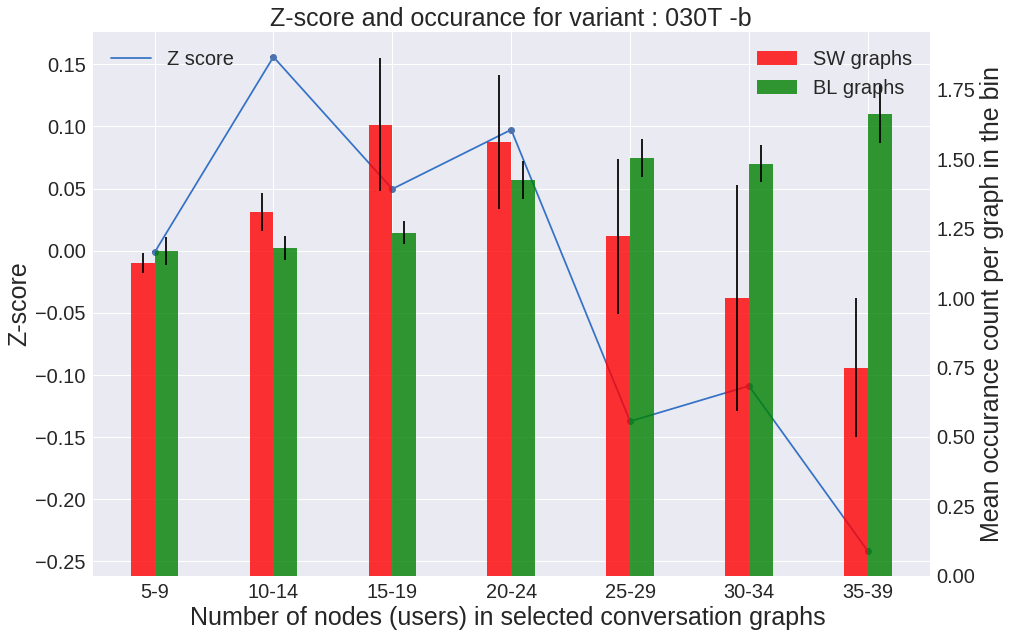
\includegraphics[width=0.33\textwidth ]{030T-b.png}
    }
    \subfloat[]{
        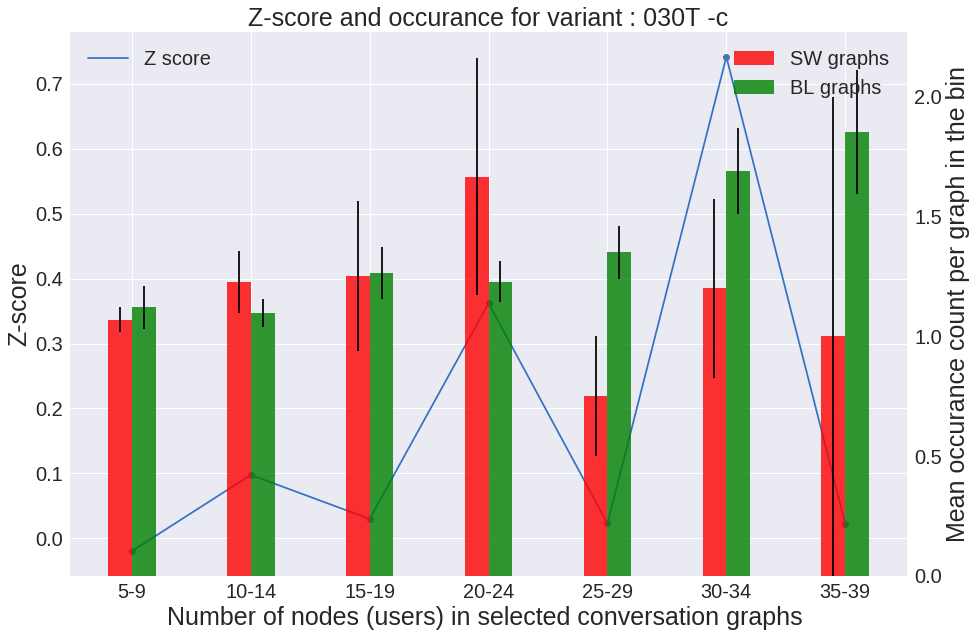
\includegraphics[width=0.33\textwidth]{030T-c.png}
    }
    
    \stepcounter{row}%
    \subfloat[]{
        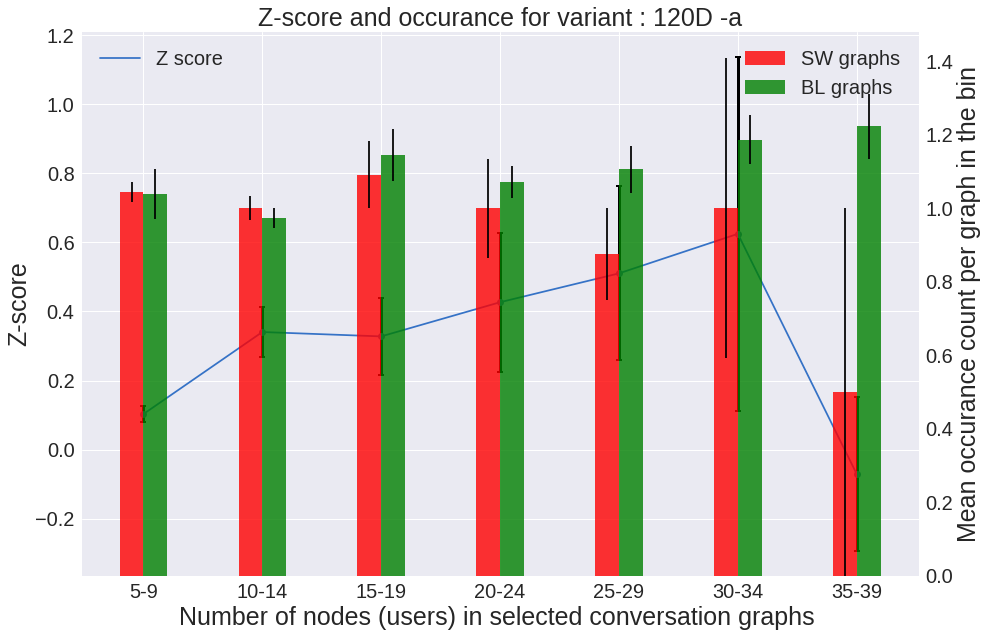
\includegraphics[width=0.33\textwidth]{120D-a.png}
    }
    \subfloat[]{
        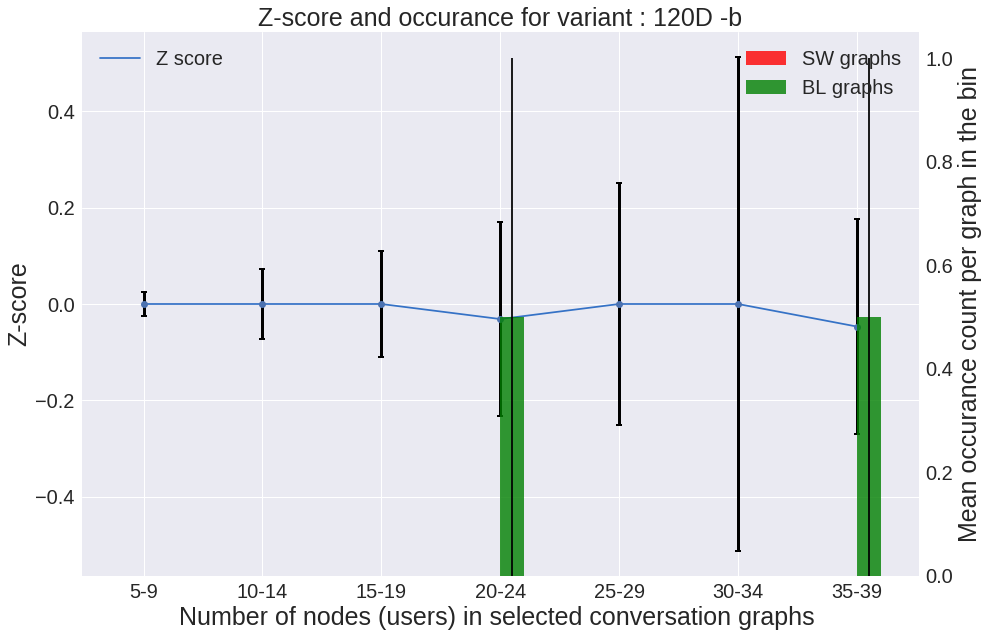
\includegraphics[width=0.33\textwidth ]{120D-b.png}
    }
    \subfloat[]{
        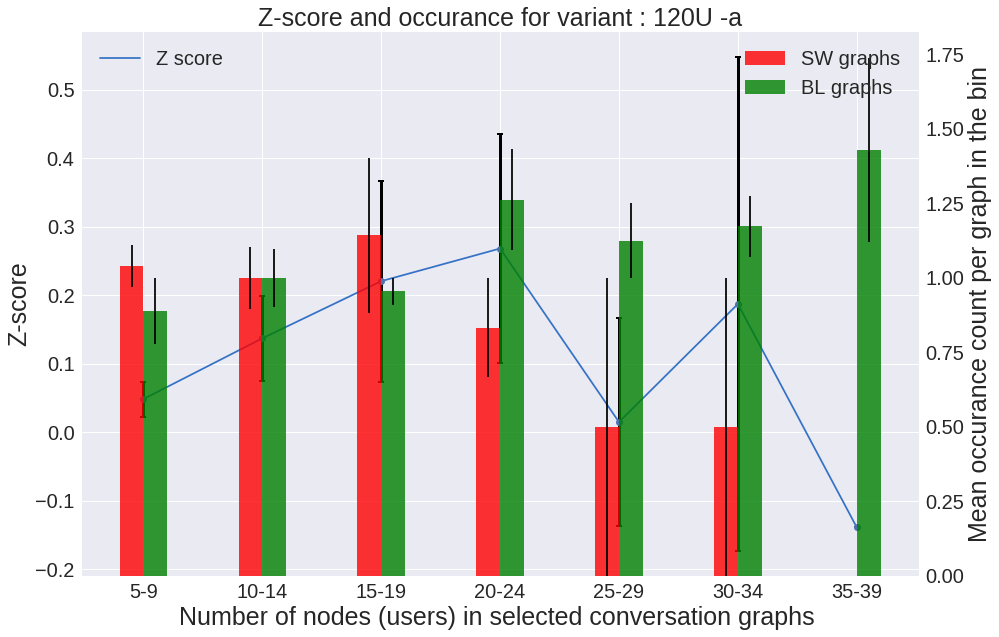
\includegraphics[width=0.33\textwidth ]{120U-a.png}
    }
    
    \stepcounter{row}%
    \subfloat[]{
        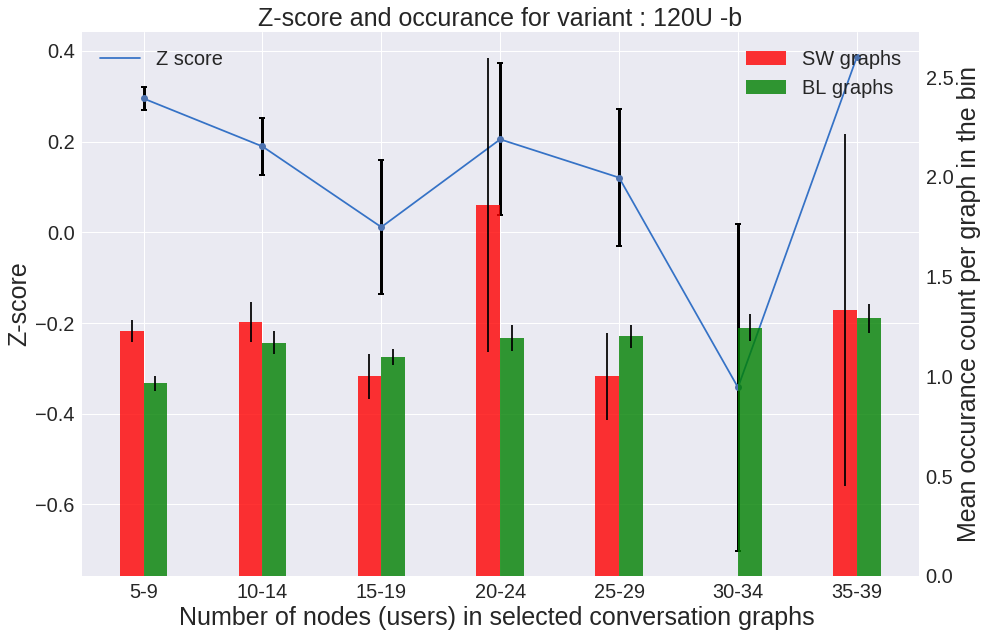
\includegraphics[width=0.33\textwidth ]{120U-b.png}
    }
    \subfloat[]{
        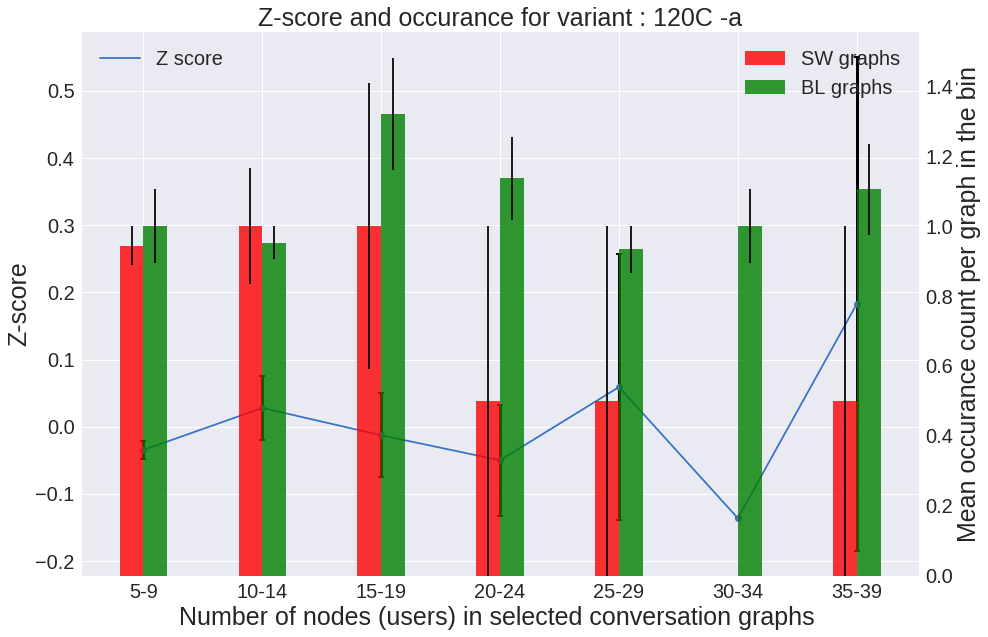
\includegraphics[width=0.33\linewidth ]{120C-a.png}
    }
    \subfloat[]{
        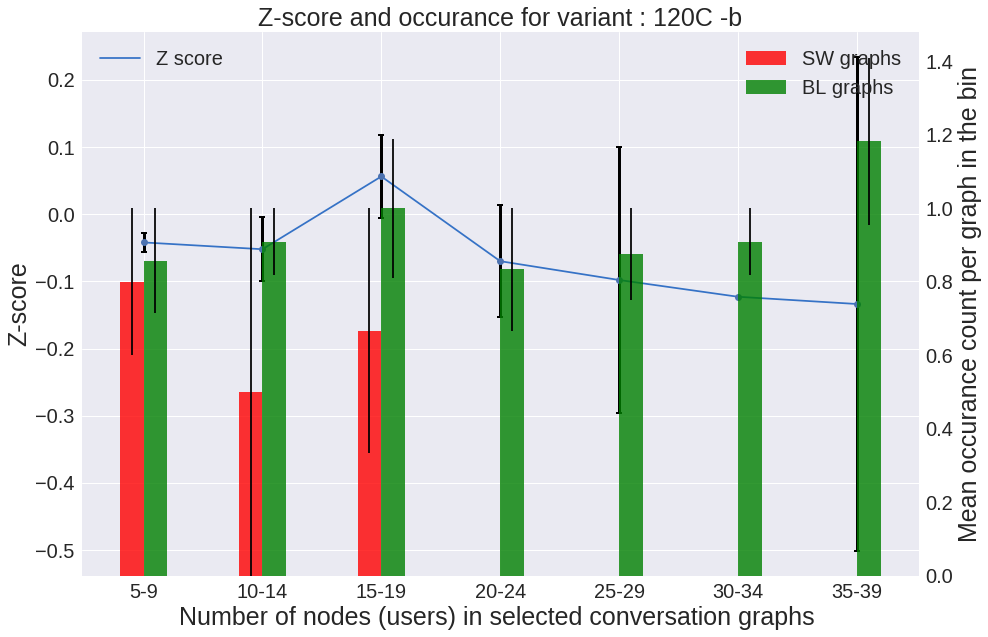
\includegraphics[width=0.33\linewidth ]{120C-b.png}
    }
    
    
    \stepcounter{row}%
    \subfloat[]{
        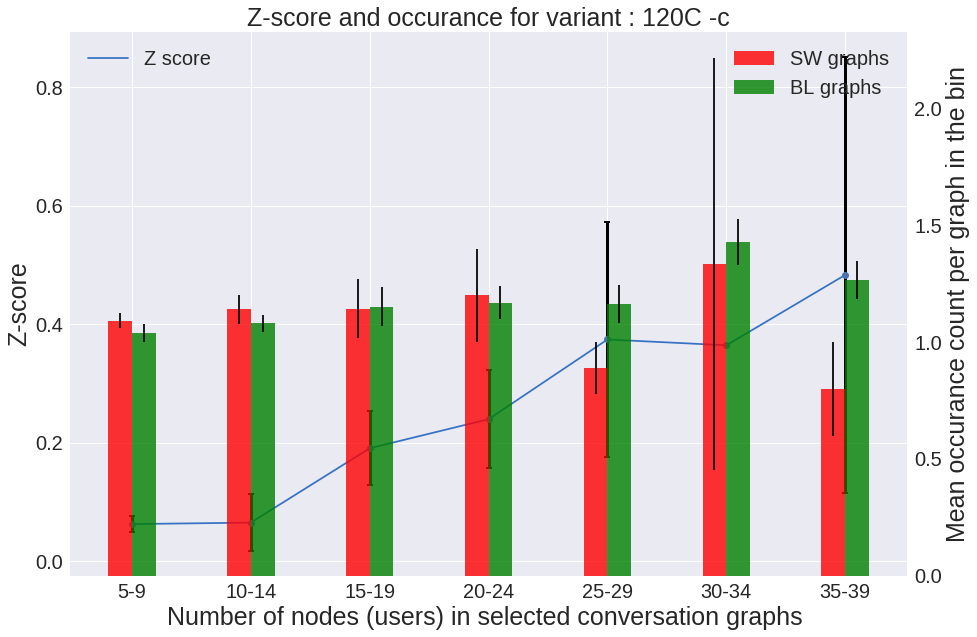
\includegraphics[width=0.33\textwidth ]{120C-c.png}
    }
    \subfloat[]{
        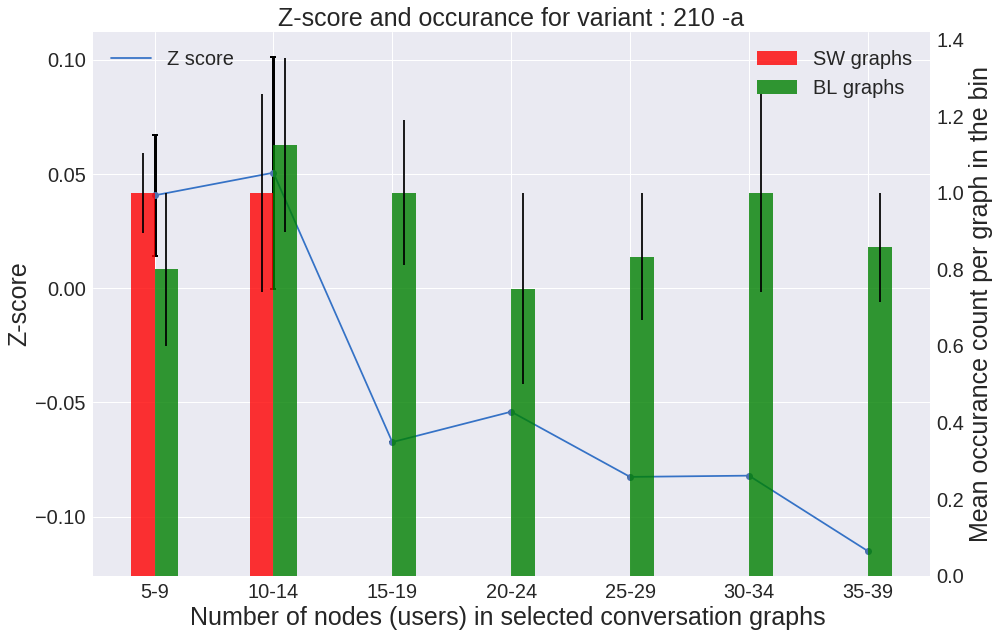
\includegraphics[width=0.33\linewidth ]{210-a.png}
    }
    \subfloat[]{
        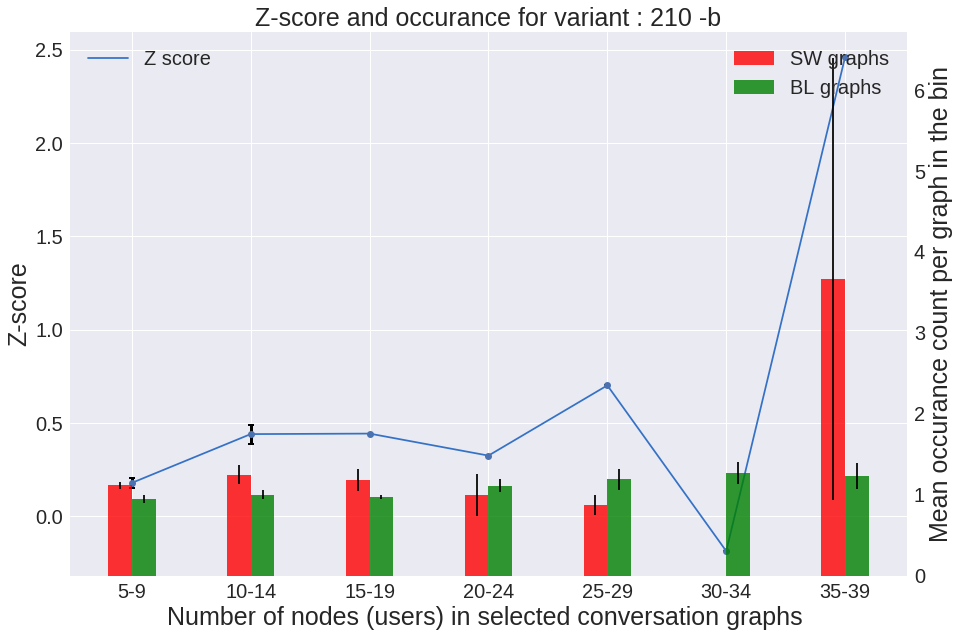
\includegraphics[width=0.33\linewidth ]{210-b.png}
    }
    
    \stepcounter{row}%
    \subfloat[]{
        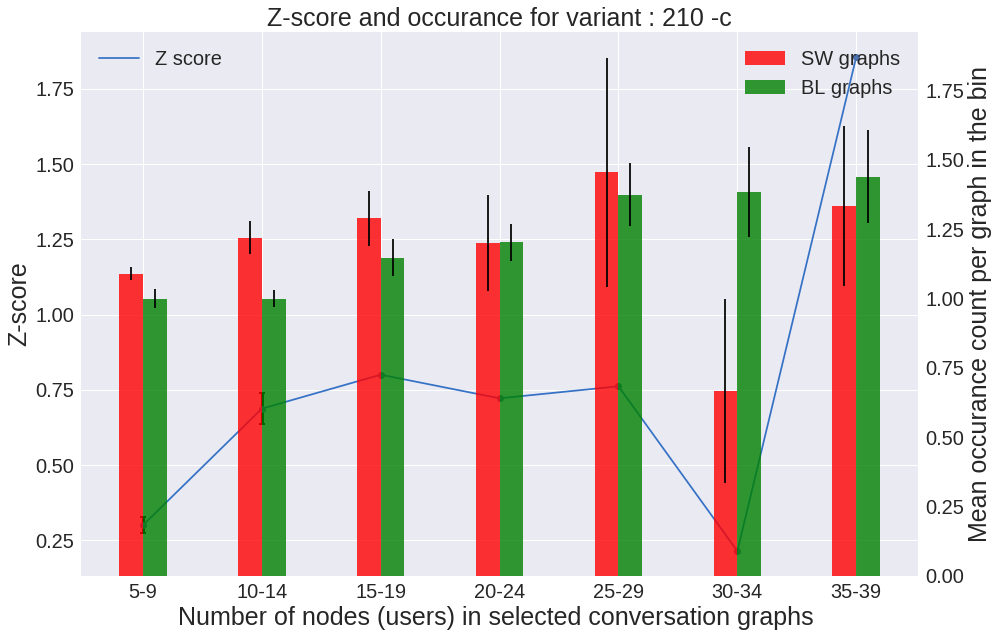
\includegraphics[width=0.33\linewidth ]{210-c.png}
    }
    
    
    \caption{ This figure lists out all the insignificant Anchored motifs, either by the virtue of rare occurance (<5 mean motifs per bin) or by account of low Z-score. }
    
    \label{fig:Rare_motifs}
\end{figure}
